
%!!! Theoretical stuff here with all needed formulas (examples are here too) !!!%

% macro for comfortable numerated formula create 
    \newcommand{\formula}[3]
    {
        \noindent#1\\[0.1cm]
        \begin{equation}\label{#2}
            #3
        \end{equation}
    }

% macro for in-text math formulas
    \newcommand{\mth}[1]
    {
        \begin{math}
            #1
        \end{math}
    }

% macro for Russian-named indexes in formulas
    \newcommand{\ruB}[1]
    {
        _{\text{#1}}
    }

\section{\Large Теоритическая часть }

\noindent\hspace{1cm}Теплопроводность — это процесс передачи тепловой энергии от нагретых частей системы к холодным за счёт хаотического движения частиц среды (молекул, атомов и т.п.). В газах теплопроводность осуществляется за счёт непосредственной передачи кинетической энергии от быстрых молекул к медленным при их столкновениях. Перенос тепла описывается законом Фурье, утверждающим, что плотность потока энергии \mth{\overline{q} \left[ \frac{\text{Вт}}{\text{м}^2} \right]} (количество теплоты, переносимое через единичную площадку в единицу времени) пропорциональна градиенту температуры \mth{\nabla T}:

\formula
{}
{Fourier}
{\overline{q} = -k \cdot \nabla T,}

\noindentгде k\mth{\left[ \frac{\text{Вт}}{\text{м}\cdot K} \right]} - коэффициент теплопроводности. \\[0.2cm]

\noindent\hspace{1cm}Молекулярно-кинетическая теория даёт следующую оценку для коэффициента теплопроводности газов:

\formula
{}
{approxK}
{k \,\, \mathtt{\sim} \,\, \lambda \overline{v}\cdot nc_{_{V}},}

\noindentгде \mth{\lambda} - длинна свободного пробега молекул газа, \mth{\overline{v} = \sqrt{\frac{8k\ruB{Б}T}{\pi m}}} - средняя скорость их теплового движения, n - концентрация (объёмная плотность) газа, \mth{c_{_V} = \frac{i}{2}k\ruB{Б}} - его теплоемкость при постоянном объёме в расчёте на одну молекулу (i - эффективное число степеней свободы молекулы). \\[0.2cm]

\noindent\hspace{1cm}Длина свободного пробега может быть оценена как \mth{\lambda = \frac{1}{n\sigma}}, где \mth{\sigma} - эффектиное сечение столкновений молекул друг с другом. Тогда из (\ref{approxK}) видно, что коэффициент теплопроводности газа не зависит от плотности газа и определяется только его температурой. В простейшей модели твёрдых шариков \mth{\sigma = const}, и коэффициент теплопроводности пропорционален корню абсолютной температуры: \mth{k \propto \frac{\overline{v}}{\sigma} \propto \sqrt{T}}. На практике эффективное сечение \mth{\sigma(T)} следует считать медленно убывающей функцией T. \\[0.2cm]

\noindent\begin{minipage}[c]{0.54\textwidth}
    \hspace{1cm}Рассмотрим стационарную теплопроводность в цилиндрической геометрии (см. рис. 1). Пусть тонкая нить радиусом \mth{r_1} и длиной L помещена на оси цилиндра радиусом \mth{r_0.} Температура стенок цилиндра \mth{T_0} поддерживается постоянной. Пусть в нити выделяется некоторая тепловая мощность Q [Вт]. Если цилиндр длинный \mth{(L >> r_0),} можно пренебречь теплоотводом через его торцы. Тогда все параметры газа можно считать зависящими только от расстояния до оси системы r. Вместо (\ref{Fourier}) имеем:
\end{minipage}
\begin{minipage}[c]{0.4\textwidth}
    \begin{center}
        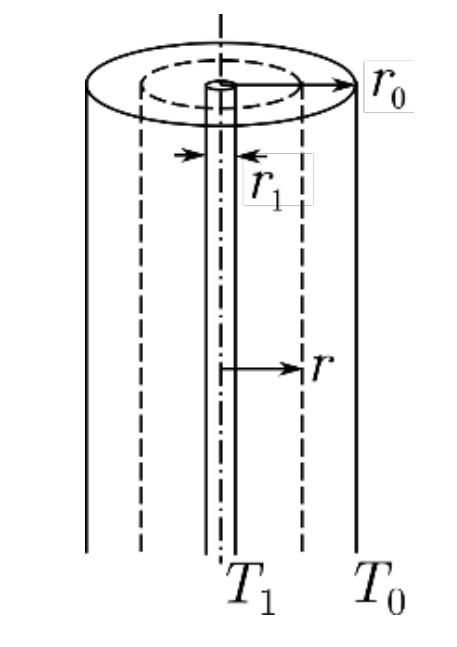
\includegraphics[scale=0.22]{picks/2_2_3_scheme1.jpg} \\
        \textit{\textcolor[HTML]{000000}{Рис. 1. Геометрия \\ задачи}}
    \end{center}
\end{minipage}

\formula
{}
{transFourier}
{q = -k\frac{dT}{dr}}

\newpage

\formula
{В стационарном состоянии полный поток тепла через любую цилиндрическую поверхность радиуса r площадью  \mth{S = 2\pi rL} должен быть одинаков и равен \mth{Q = qS}:}
{formQ}
{Q = -2\pi rL\cdot k\frac{dT}{dr} = const}

Если перепад температуры  \mth{\Delta T = T_1 - T_0} между нитью и стенками цилиндра мал \mth{(\Delta T << T_0),} то в (\ref{formQ}) можно пренебречь изменением теплопроводности от температуры в пределах системы, положив \mth{\chi \approx \chi(T_0)}. Тогда разделяя переменные в (\ref{formQ}) и интегрируя от радиуса нити до радиуса колбы получим:

\formula
{}
{finalQ}
{Q = \frac{2\pi L}{ln\frac{r_0}{r_1}} k\cdot \Delta T}

\vspace{1cm}

\begin{center}
    {\bf\Large
    Схема установки:}
    
    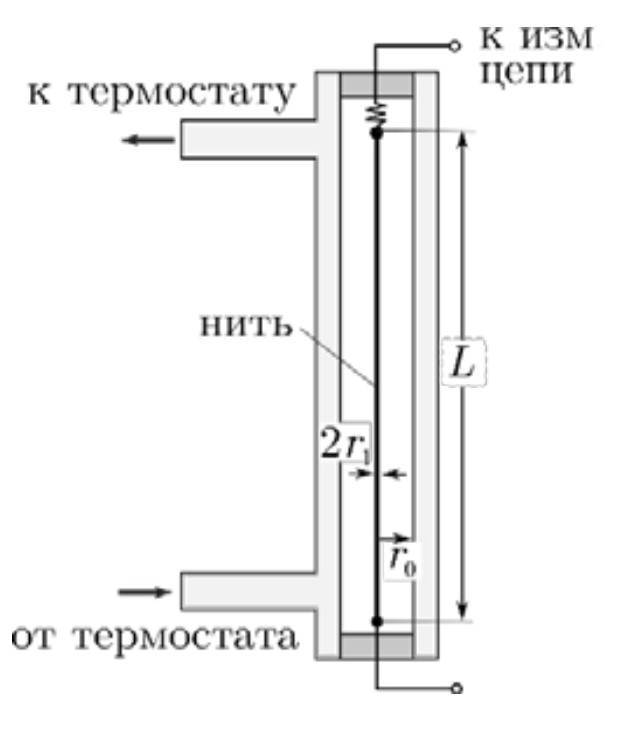
\includegraphics[scale=0.5]{picks/2_2_3_scheme2.jpg} \\
    \textit{\textcolor[HTML]{000000}{Рис. 2. Схема установки}}
    
\end{center}

\newpage